\newpage
\subsection*{Aufgabe 27}
\begin{wrapfigure}{L}{8cm}
  \centering
  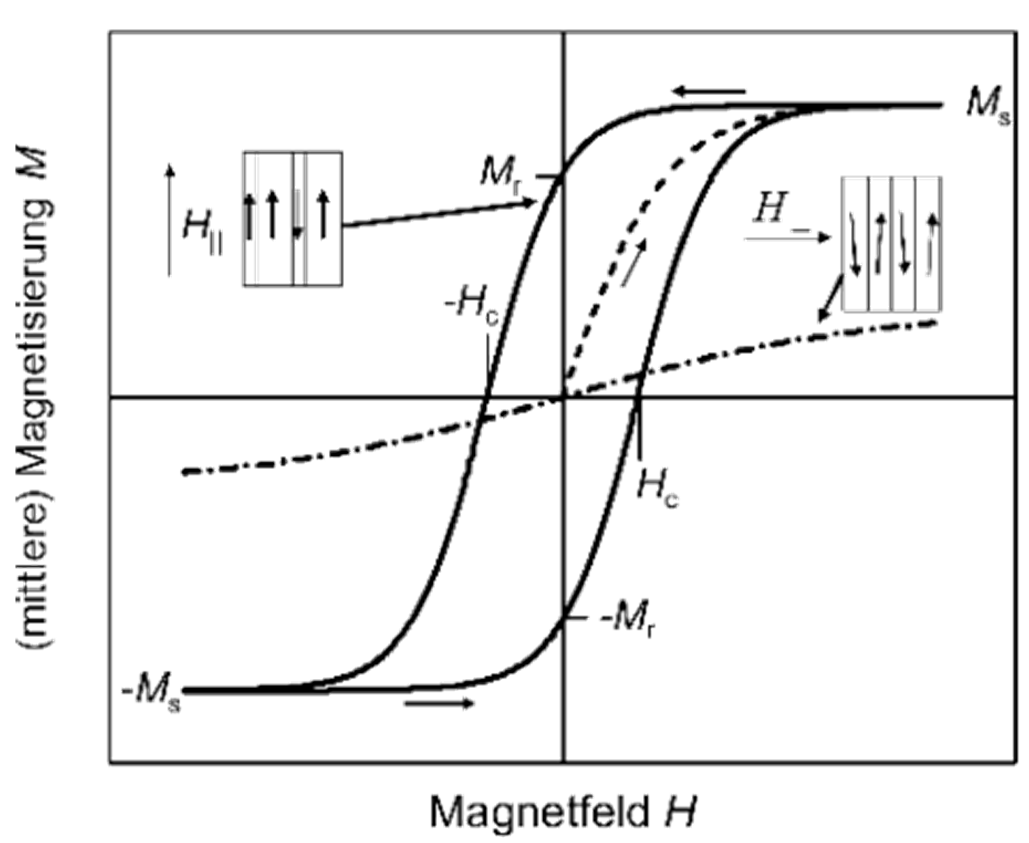
\includegraphics[width=8cm]{aufgabe27.png}
\caption{Dem Skript entnommen.}
\end{wrapfigure}
\subsubsection*{a)}
Sättigungsmagnetisierung $M_S$: Die maximal mögliche Magnetisierung.
Remanenz $M_R$: Die nach Abschalten von $H$ verbleibende Magnetisierung.
Koerzitiv-Feldstärke $H_C$ : Die Feld-stärke (in Gegenrichtung) bei der eine
vorhandene Magnetisierung verschwindet.

\subsubsection*{b)}
"`Leichte"' Richtung (z.B Stabmagnet): Durchgezogene Linie. "`Schwere"' Richtung
(dünner Film mit Magnetisierung senkrecht zur Oberfläche): Gestrichelte Linie:
Keine Hysterese.\newline Warum ???
